\section{Theoretical Foundations}

In the following section, the theoretical foundations of keystroke dynamics are going to be explained. First, the type of texts that can be used for the feature extraction phase is going to be explained. Then, the features that are going to be extracted from the text are going to introduced. Finally, the different algorithms that are going to be used are going to be explained along with some characteristics of biometric systems that can be used to evaluate the performance of each algorithm.

\subsection{Data extraction}

It is possible to define two types of text that can be used for feature extraction:

\begin{itemize}
	\item Fixed text: This type of text is the one that is written by the user using a fixed source. It is generally a short phrase or a word that is used to identify the user. A good example of this type of text is the password and username that are employed to log into a computer or a website.

	\item Free text: This type of text is the one that is written by the user without any restriction. This kind of text is the most common in the real world but it is generally the most difficult to analyze because of the lack of restrictions and the introduction of important factors like, the user's level of concentration, thinking time, etc.
\end{itemize}



\subsection{Features}

In general, the features extracted from the keystroke dynamics are based on the study and analyzes data involving digraphs and trigraphs. In the keystroke dynamics literature a digraph is a set of two consecutive characters that represents two keystrokes, that can be letters, numbers or symbols and other keys that do not necessarily represent a language character like the space bar, shift key or enter key. Logically, a trigraph is a set of three consecutive characters that represents three keystrokes \cite{trigraphs}. Some of the most common features that can be extracted from a single keystroke, a digraphs or a trigraphs are the following \cite{monrose2000keystroke, machine_learning}:

\begin{itemize}
	\item Tap timestamp: Defined as the timestamp of the key press.
	\item Release timestamp: Defined as the timestamp of the key release.
	\item Time between keystrokes: This feature is commonly defined as the time that elapses between the key press of the first keystroke and the key release of the second keystroke of a digraph or trigraph.
	\item Hold time: This is defined as the time that elapses between the key press and the key release of a keystroke.
	\item Words per minute (WPM): This is the average number of words that a user can type in a minute.
	\item Percentage of usage of special keys: This feature is defined as the percentage of times that a user uses keys like the shift key or Caps-Lock key.
\end{itemize}

\subsection{Classification techniques}

Once the features are extracted, the next step is to use algorithms to authenticate the user. Most of these techniques can be classified into two groups.


The first group is based on the usage of distance metrics. These set of techniques are take use of the calculation of the distance between the features of the user that is trying to be identified and the features of the users that are already registered in the system. Features are displayed as a vector of multiple dimensions and the distance between vectors is calculated using a distance metric. Some metrics that can be used are the Manhattan distance and the Mahalanobis distance.

On one hand, Manhattan distance for $n$ dimensions can be defined as the sum of the absolute differences between the coordinates of the vectors, As represented in the following formula:

\begin{equation}
	d(x,y) = \sum_{i=1}^{n} |x_i - y_i|
	\label{eq:manhattan}
\end{equation}

Where $x$ and $y$ are vectors of $n$ dimensions and $x_i$ and $y_i$ are the $i$th coordinates of the vectors $x$ and $y$ respectively.

On the other hand Mahalanobis distance can be defined as the distance between two points that depends on the probability distribution of all the points \cite{de2000mahalanobis}. The squared version of this distance can be described by the following formula:

\begin{equation}
	d(x,y) = (x-y)^T S^{-1} (x-y)
	\label{eq:mahalanobis}
\end{equation}

Where $x$ and $y$ are vectors of $n$ dimensions and $S$ is the covariance matrix of the set of points.


These distances are commonly used in clustering algorithms like K-nearest neighbors. This algorithm stores the multidimensional feature vectors such that when a vector is received it can be classified by the majority of the classes of the nearest neighbors using a distance metric. In the user authentication problem, the user can be identified by finding the single nearest neighbor and using a threshold to determine if the user is the same as the one that is trying to be identified. A simple knn example for 2 dimensional features can be shown in figure \ref{fig:knn}.

\begin{figure}[h]
    \centering
    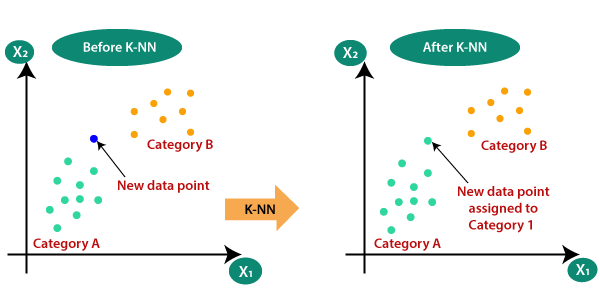
\includegraphics[width=0.7\linewidth]{images/knn}
    \caption{K-nearest neighbors algorithm \cite{knn}}
    \label{fig:knn}
\end{figure}

The second group of techniques is based on the use of deep learning techniques.

One of the most important parts of this approach is the use of algorithms to vectorize the text, such that said text can be used as input for the neural network. Some of the most common vectorization techniques try to represent text as numbers, assigning numeric values to words, characters or more complex structures like tokens. Other techniques try to transform images into matrices that contain RGB or grayscale values of the pixels. Finally there are techniques that have numbers as input and try to normalize and standardize the data to perform better in the neural network.

This techniques are characterized by the use of neural networks. These networks try to simulate the human brain by being composed of multiple layers of neurons that are connected to each other. Each neuron is a mathematical function that receives multiple inputs and produces one or more outputs.

The neural networks that are going to be used in this project are the following:

\begin{itemize}
	\item Convolutional Neural Networks: CNNs are a type of neural network architecture that have been successful in tasks such as image classification, object detection, image segmentation, by feature extraction. \cite{valueva2020cnn}. They are designed to automatically learn and extract hierarchical patterns and features from input data. CNNs use convolutional layers, pooling layers, and fully connected layers \cite{taye2023layers}. Convolutional layers apply filters to the input data, capturing spatial dependencies and detecting local patterns. Pooling layers reduce the spatial dimensions of the data. Fully connected layers are usually placed at the end of the network and are used to get the final output.
	\item Recurrent Neural Network: RNNs are neural network architectures suitable for sequential data such as time series, text, and speech\cite{li2015rnn_structure}. Unlike traditional networks, RNNs contain loops that allow information to persist and be processed across different time steps \cite{dupond2019rnn}. The presence of a hidden state, the internal memory of the network, grants RNNs the ability to capture temporal dependencies and contextual information within the data.
	\item Gated Recurrent Unit: GRU is a variation of RNN designed to address the vanishing gradient problem and improve the modeling of long-term dependencies. GRU incorporates gatelike mechanisms that regulate the flow of information within the network. GRU units consist of an update gate and a reset gate, which control the operations of information update and reset in the hidden state \cite{cho2014gru}. The update gate determines how much of the previous hidden state to retain, while the reset gate decides how much of the previous state to forget. GRUs have demonstrated superior performance over traditional RNNs in various tasks such as language modeling, machine translation, and speech recognition \cite{ravanelli2018gruperformance}.
\end{itemize}

\subsection{benchmark}

The following factors are used to evaluate the performance of biometric systems \cite{benchmarks}:

\begin{itemize}
	\item False Acceptance Rate (FAR):
	FAR is a metric used in biometric system benchmarking to measure the likelihood of the system incorrectly granting access to unauthorized individuals. It represents the rate at which the system mistakenly identifies impostors as genuine users. A lower FAR indicates a higher level of security, as it means the system is less likely to mistakenly accept unauthorized individuals. This characteristic can be represented by the following formula:

	\begin{equation}
		FAR = \frac{\text{False Acceptances}}{\text{Total Impostor Attempts}}
		\label{eq:far}
	\end{equation}
	
	\item False Rejection Rate (FRR):
	FRR is a metric used to assess the probability of the biometric system incorrectly rejecting legitimate users. It represents the rate at which the system fails to recognize or authenticate genuine users. A lower FRR indicates better user convenience, as it means the system is less likely to deny access to legitimate users. This metric can be represented by the following formula:
	\begin{equation}
		FRR = \frac{\text{False Rejections}}{\text{Total Genuine Attempts}}
		\label{eq:frr}
	\end{equation}
	
	\item Equal Error Rate (EER):
	EER is a benchmark point where the FAR and FRR are equal as seen in Figure \ref{fig:eer}. It signifies the threshold or decision boundary at which the system achieves a balance between false acceptances and false rejections. The EER provides a summary measure of the system's performance and is commonly used for comparing different biometric systems. A lower EER indicates better overall performance, as it reflects a balanced trade-off between security and user convenience.
	\begin{figure}[h]
	    \centering
	    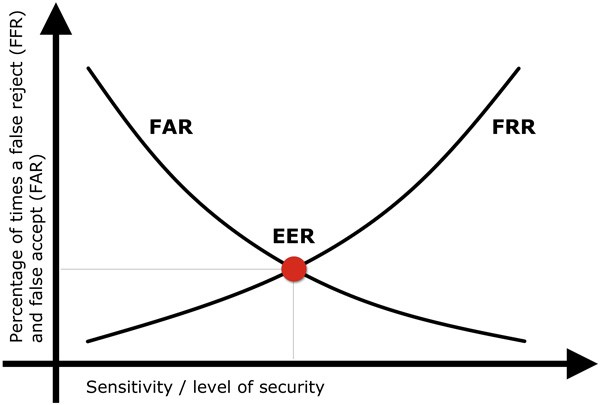
\includegraphics[width=0.7\linewidth]{images/eer}
	    \caption{Equal Error Rate \cite{eer}}
	    \label{fig:eer}
	\end{figure}
\end{itemize}